\chapter[Gerência de Requisitos]{Gerência de Requisitos}

\section{Nível de Portifólio}

A camada de Portfólio consiste no nivel mais elevado do SAFe, onde programas sao alinhados à
estratégia de negócios da empresa ao longo de linhas da corrente de valor. No presente trabalho,
o nivel de portfólio é destacado a partir das atividades \textbf{Entender o Contexto do Cliente},
\textbf{Levantar Epicos} e \textbf{Selecionar e detalhar épicos} que foram realizadas utilizando as
técnicas de elicitação, workshops e entrevistas. As atas de reunião, jutamente com as entrevistas,
podem ser encontradas no apêndice \ref{apendice:brainstorms}.

\subsection{Requisitos Identificados}

\textbf{Tema de Investimento:} Gestão da Manutenção

Extraido a partir das prioridades da organização, serve para assegurar que o desenvolvimento
do software estará de acordo com a estrategia da organização.

Dado que o gargalo identificado na gestão da manutenção de sistemas do MC e onde o cliente irá investir.
Cada épico foi detalhado utilizando o template de lightweight business case, recomendado pelo SAFe. \cite{scaleP}

\textbf{Épico 01:} EP-01 Gerenciamento de Demandas

Abrange todo o movimento das demandas em torno do fluxo estabelecido, desde sua criacao ate o seu fechamento.

\begin{table}[]
\centering
\caption{Épico 1}
\label{my-label}
\begin{tabular}{|c| p{13cm} |}
\hline
\multicolumn{2}{|c|}{Caso de Negócio}                                                                                                                \\ \hline
Para                 & O gerente e a equipe de desenvolvimento                                                                                       \\ \hline
Quem                 & Gere e desenvolve as demandas aprovadas de manutenção do ministério                                                           \\ \hline
A                    & Ferramenta de Gestão do Desenvolvimento                                                                                       \\ \hline
É uma                & Ferramenta que organiza sistematicamente a demanda a ser desenvolvida                                                         \\ \hline
Que                  & Facilita e Agiliza o trabalho da equipe de desenvolvimento                                                                    \\ \hline
Diferente            & Da situação atual que tudo é feito manualmente                                                                                \\ \hline
Nossa Soluação       & Automatiza a gestão e Centraliza as informações das demandas a serem desenvolvidas                                            \\ \hline
\multicolumn{2}{|c|}{Escopo}                                                                                                                         \\ \hline
Critérios de Sucesso & \begin{tabular}[c]{@{}c@{}}Produtividade aumentar em 100\%\\ \\ Demandas aprovadas pelo usuário aumentar em 20\%\end{tabular} \\ \hline
No Escopo            & Controle de demandas por parte do Gestor.                                                                                     \\ \hline
Fora do Escopo       & \begin{tabular}[c]{@{}c@{}}Validação de demandas.\\ Registro de demanda por parte do cliente.\end{tabular}                    \\ \hline
\end{tabular}
\end{table}

\textbf{Épico 02:} EP-02 Gerenciamento de Usuários

Interfere no modo de comunicacao entre o usuario e o sistema, considerando diversos aspectos referente ao seu acesso.

\begin{table}[H]
\centering
\caption{Épico 2}
\label{epic:segundo}
\begin{tabular}{|c| p{13cm} |}
\hline
\multicolumn{2}{|m{4cm}|}{\textbf{Caso de Negócio}} \\ \hline
  Para   &   O gerente e a equipe de desenvolvimento        \\ \hline
  Quem         &    Gere e desenvolve as contas de usuário        \\ \hline
    A       &     Ferramenta de Gestão do Manutenção    \\ \hline
      É uma     &    Ferramenta que organiza sistematicamente a demanda a ser desenvolvida \\ \hline
      Que     &     Facilita e Agiliza o trabalho da equipe de desenvolvimento \\ \hline
      Diferente   &     Da situação atual que tudo é feito manualmente     \\ \hline
      Nossa Soluação  &   Automatiza a gestão e Centraliza as informações das demandas a serem desenvolvidas    \\ \hline
\multicolumn{2}{|l|}{Escopo} \\ \hline
Critérios de Sucesso  &  Produtividade aumentar em 100\% e Demandas aprovadas pelo usuário aumentar em 20\%    \\ \hline
No Escopo & Controle de demandas por parte do Gestor. \\ \hline
Fora do Escopo  & Validação de demandas. e Registro de demanda por parte do cliente.     \\ \hline
\end{tabular}
\end{table}

\section{Nível de Programa}

A camada de Programa consiste na camada intermediária do SAFe, onde tem uma relação
direta com o nível de time e o planejamento das iterações. No presente trabalho,
o nivel de programa foram executadas as seguintes atividades: eh destacado a partir das atividades:

\begin{itemize}
  \item Leventar Requisitos não funcionais
  \item Selecionar épicos para iteração,
  \item Levantar features
  \item Levantar histórias de usuário
  \item Planejar Releases
  \item Gerenciar Mudanças
\end{itemize}

\subsection{Requisitos não funcionais}

Os requisitos não funcionais identificados se encontram no documento de visão que se encontra no apendice
[apendice]. Neles foram especificadas regras como níveis de usuário de acesso entre outras restrições
que contribuiram também para elicitar os requisitos da próxima sessão.

\subsection{Requisitos identificados}

Considerando as atividades do processo, foram levantadas as features e suas
respectivas histórias, para obter uma melhor estimativa no planejamento das releases,
nesta sessão serão descritas apenas as features levantadas, as histórias se encontram

\textbf{Feature 1:} Manutenção de Usuários

Esta feature tem como objetivo manter os usuários do sistema, permitindo o cadastro,
definição de tipo de conta, cadastro de usuários e edição dos mesmos.

\textbf{Feature 2:} Acesso de Usuários

Essa feature tem como objetivo o controle da sessão dos usuários permitindo os
mesmos se `logar` no sistema e recuprar sua senha.


\textbf{Feature 3:} Acompanhamento de Demandas
Essa feature tem como objetivo prover as funcionalidades para
que os stakeholders consigam acompanhar as demandas e visualizar
as mesmas de acordo com o seu nível de usuário.


\textbf{Feature 4:} Manutenção de Demandas
Essa feature tem com oobjetivo a manutenção das demandas e atualização das
demandas seguindo o workflow de trabalho da equipe de manutenção. Proverá
a possibilidade de mudar status e responsável sobre as demandas.

\subsection{Visão}

Você deve pensar sobre grandes coisas enquanto você está fazendo coisas pequenas, garantindo que
todas as pequenas coias estão indo na direção certa
\cite{alvin}. Uma frase detalhada na descrição do documento de visão no SAFe,
que, descreve o Documento de visão como um documento que descreve uma explanação sobre a
solução a ser desenvolvida, com os requisitos não funcionais, necissdads dos stakeholders e
um resumo do contexto do sistema. O documento de visão produzido se encontra no apêndice \ref{apendices:visao}
e foi bem utilizado como passo para as próximas atividades.

\subsection{Roadmap}

O Roadmap serve como um documento que padroniza a comunicação entre o nível de time o programa,
é como um caminho que deve ser seguido em uma linha do tempo das entregas que devem ser realizadas.
Representa de 3 a 6 meses de Iterações. Representa os incrementos do software que devem ser entregues.
Existem dois tipos de Roadmap: \cite{scaleR}

\begin{itemize}
  \item \textbf{síncrono:} features são entregue sincronizadas, em cada release é entregue uma feature completa.
  \item \textbf{asincrono:} features são entregues por versões, uma release não precisa conter uma feature completa,
   mas sim uma versão que pode ser incrementada, na próxima release.
\end{itemize}

O planejamento atual, foi realizado usando o roadmap asincrono, como representado na imagem abaixo

\begin{figure}[H]
    \centering
	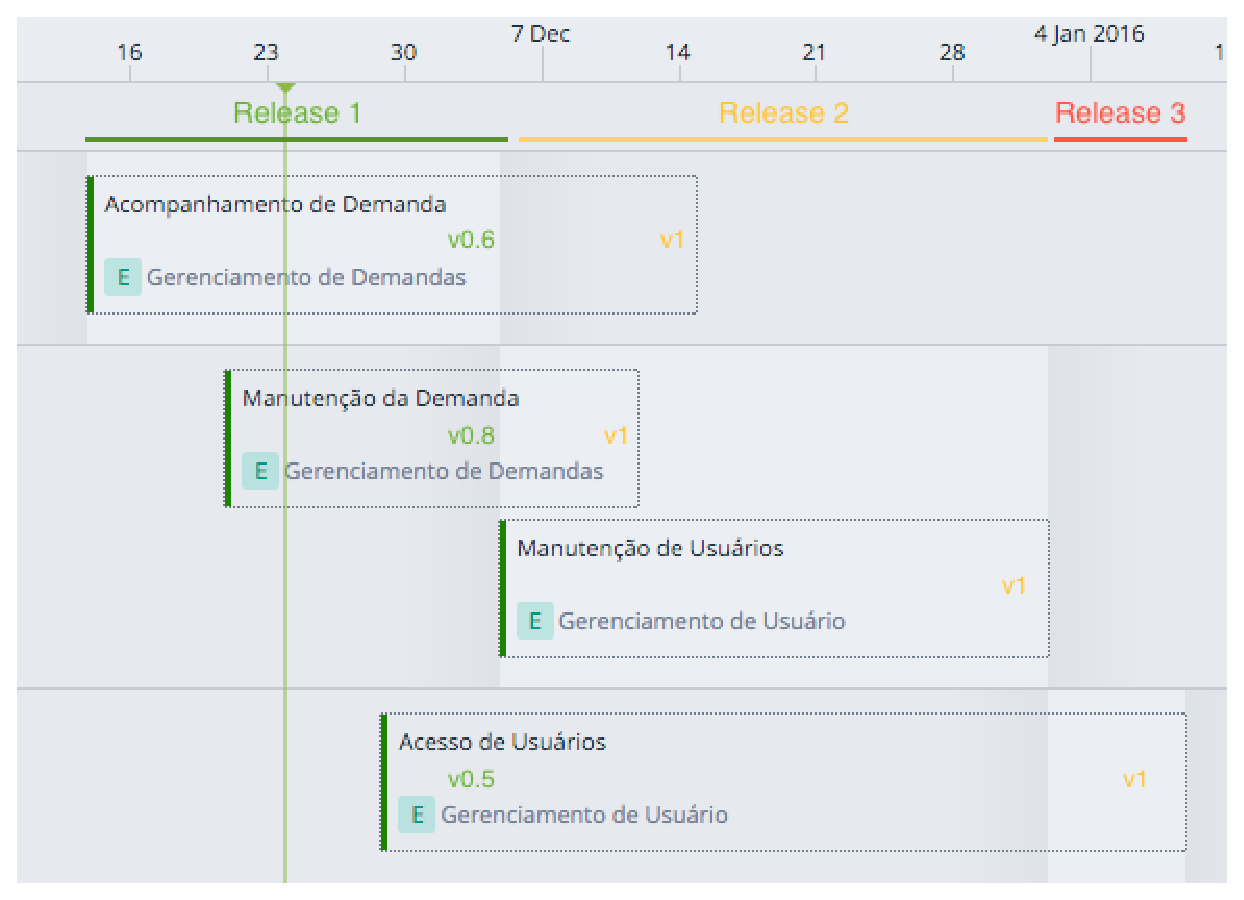
\includegraphics[keepaspectratio=true,scale=0.7]{figuras/roadmap.eps}
    \caption{Roadmap planejado}
    \label{fig:roadmap}
\end{figure}

Como descrito na imagem ,a Feature \"Acompanhamento de demenda\", na release 1.
será lançada uma v0.6 com 60\% das suas funcionalidades implementadas e a versão
final será entregue na Release 2. Respectivamente aconterá o mesmo com as outras features.

\section{Nível de Time}

Conhecido como team ágil representa o nível mais baixo do safe, no processo estabelecido,
foram realizadas as seguintes atividades do nível de time:

\begin{itemize}
  \item Detalhar histórias de usuário
  \item Levanter e priorizar necessidades do time.
  \item planejar sprints.
  \item Desenvolver sprints.
  \item Retrospectiva da sprint.
\end{itemize}

\subsection{Requisistos Identificados}

Durate a \textbf{primeira} iteração do nível de programa, foram especificadas as seguintes histórias

\begin{figure}[H]
    \centering
	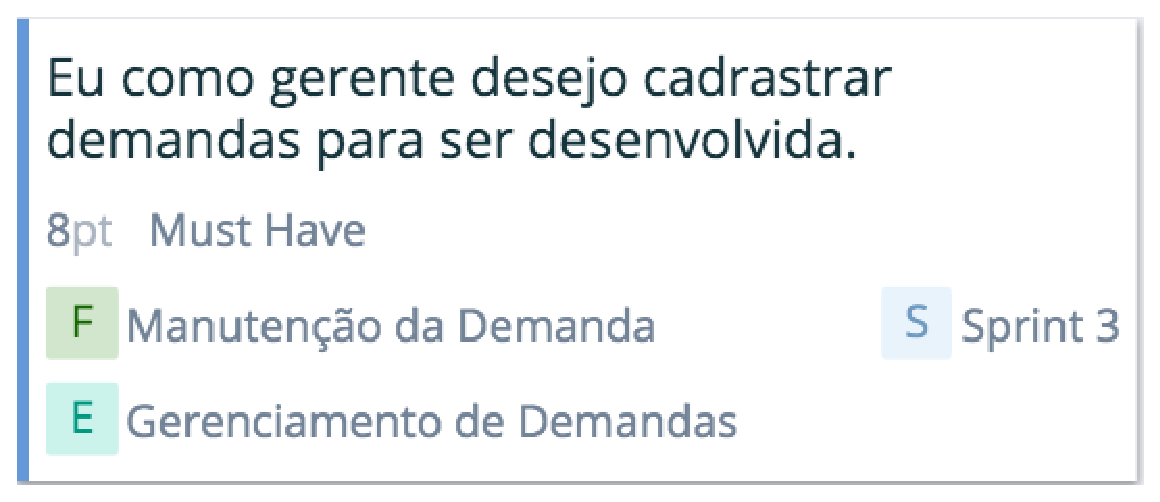
\includegraphics[keepaspectratio=true,scale=0.5]{figuras/time1.eps}
    \caption{História de Usuário 1}
    \label{fig:roadmap}
\end{figure}

\begin{figure}[H]
    \centering
	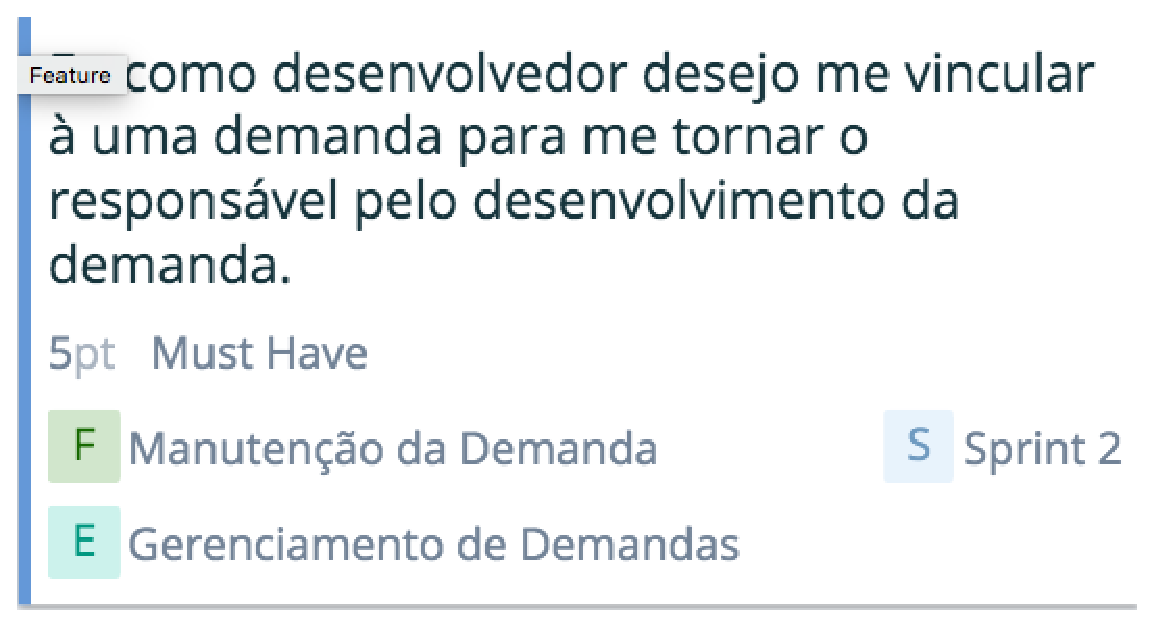
\includegraphics[keepaspectratio=true,scale=0.5]{figuras/time2.eps}
    \caption{História de Usuário 2}
    \label{fig:roadmap}
\end{figure}

\begin{figure}[H]
    \centering
	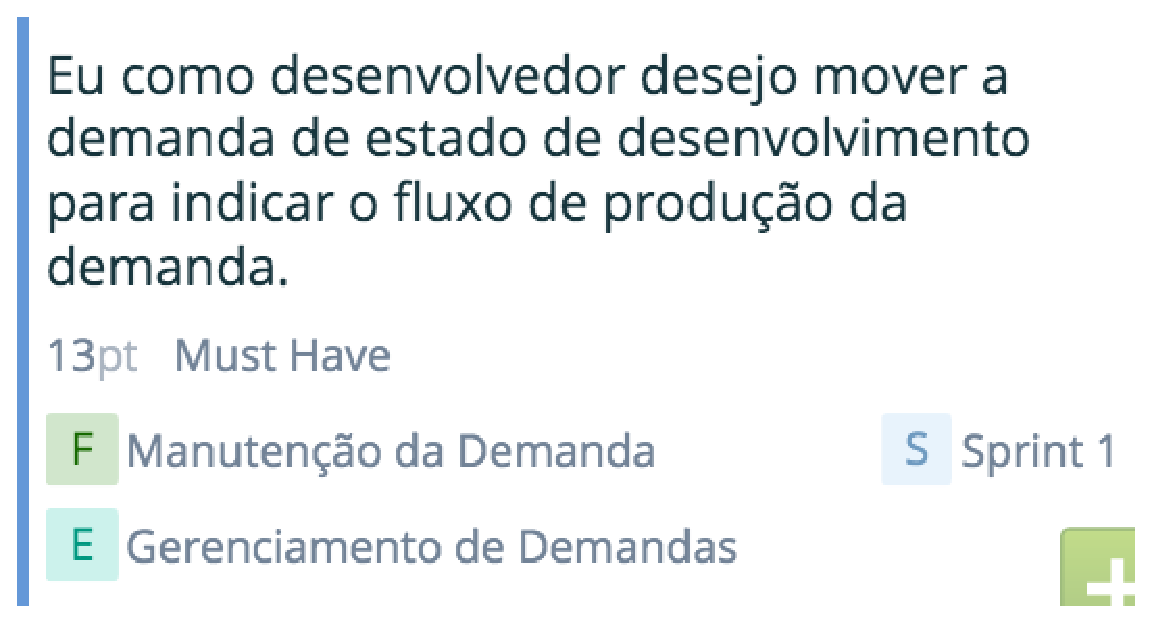
\includegraphics[keepaspectratio=true,scale=0.5]{figuras/time3.eps}
    \caption{História de Usuário 3}
    \label{fig:roadmap}
\end{figure}

\begin{figure}[H]
    \centering
	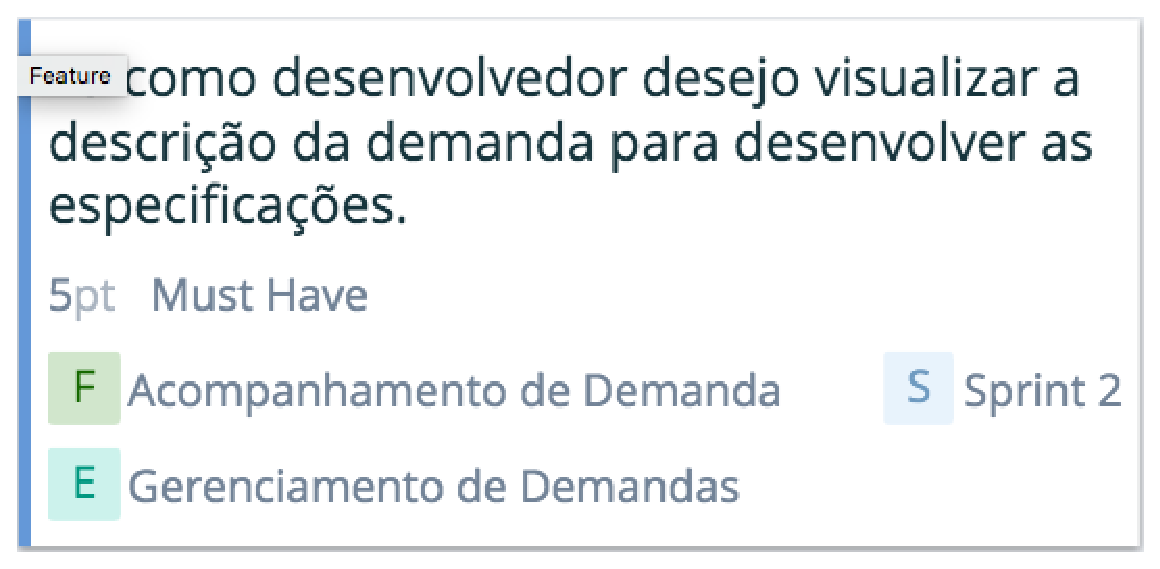
\includegraphics[keepaspectratio=true,scale=0.5]{figuras/time4.eps}
    \caption{História de Usuário 4}
    \label{fig:roadmap}
\end{figure}

\begin{figure}[H]
    \centering
	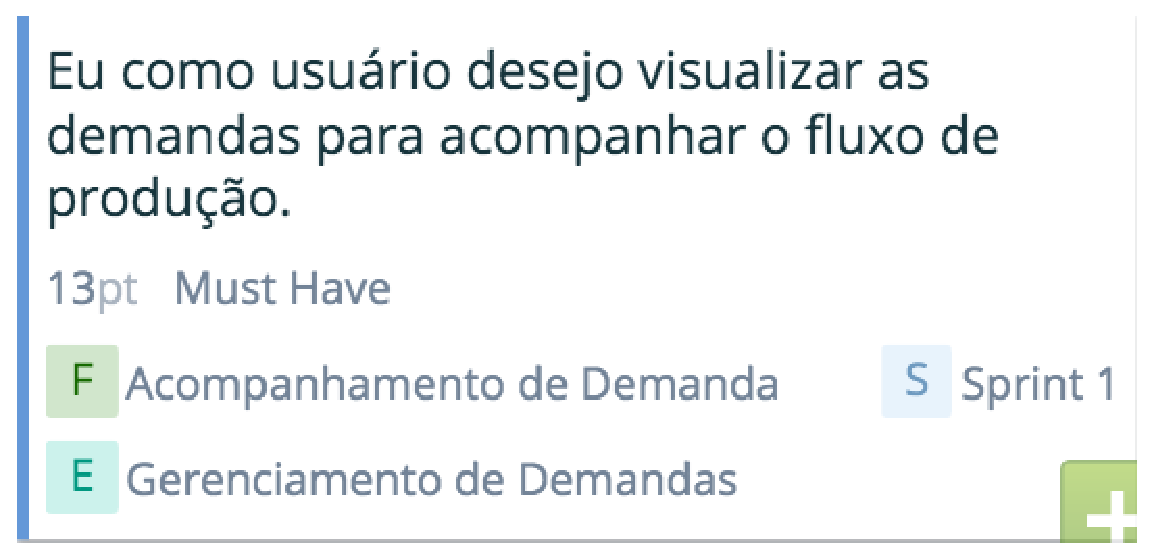
\includegraphics[keepaspectratio=true,scale=0.5]{figuras/time5.eps}
    \caption{História de Usuário 5}
    \label{fig:roadmap}
\end{figure}

\begin{figure}[H]
    \centering
	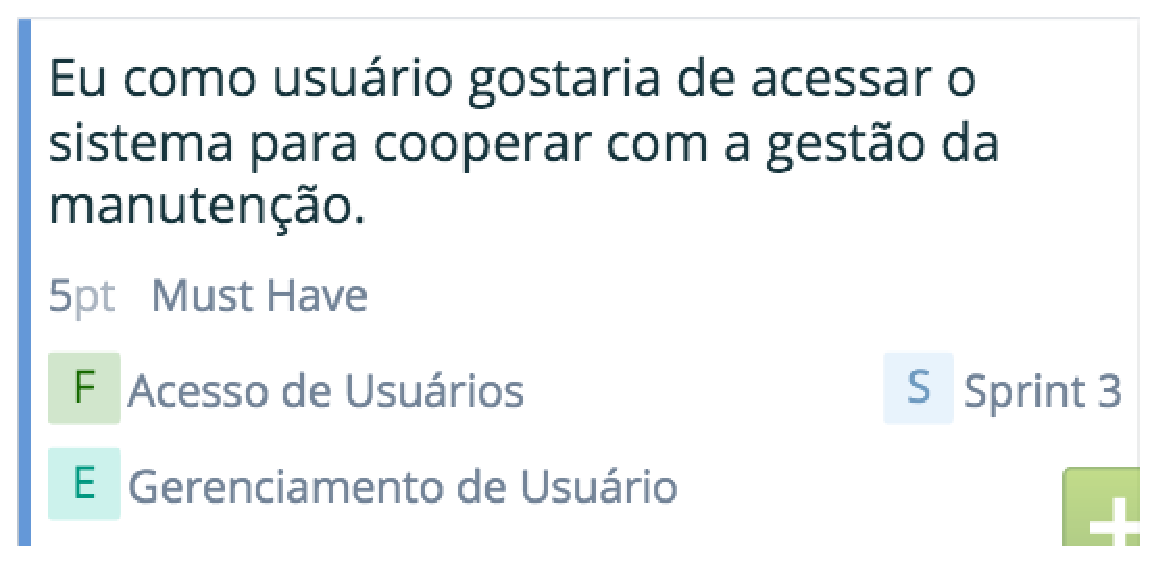
\includegraphics[keepaspectratio=true,scale=0.5]{figuras/time6.eps}
    \caption{História de Usuário 6}
    \label{fig:roadmap}
\end{figure}

Durate a \textbf{segunda} iteração do nível de programa, foram especificadas as seguintes histórias

\begin{figure}[H]
    \centering
	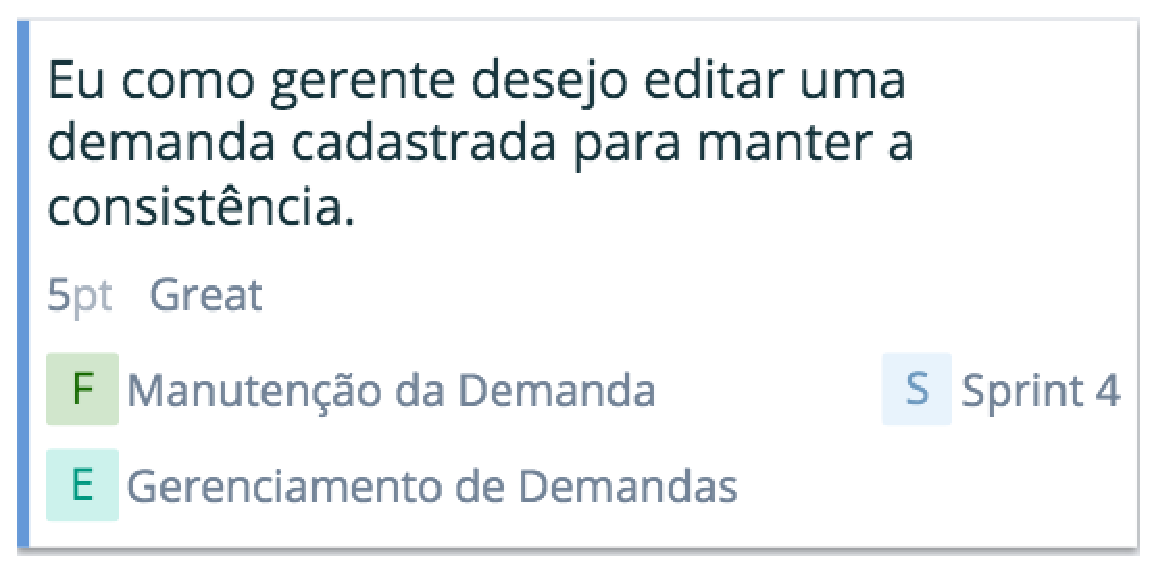
\includegraphics[keepaspectratio=true,scale=0.5]{figuras/time7.eps}
    \caption{História de Usuário 7}
    \label{fig:roadmap}
\end{figure}

\begin{figure}[H]
    \centering
	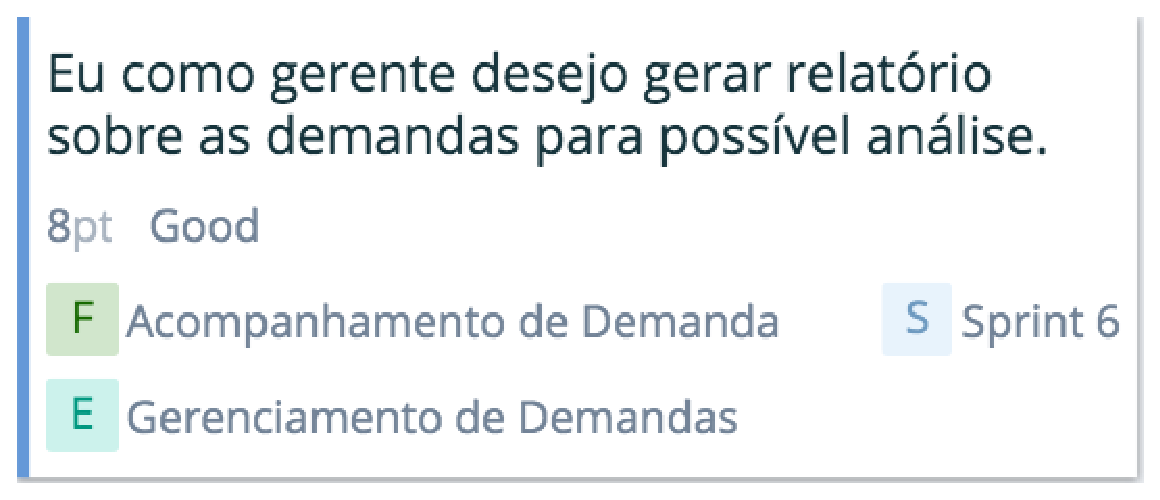
\includegraphics[keepaspectratio=true,scale=0.5]{figuras/time8.eps}
    \caption{História de Usuário 8}
    \label{fig:roadmap}
\end{figure}

\begin{figure}[H]
    \centering
	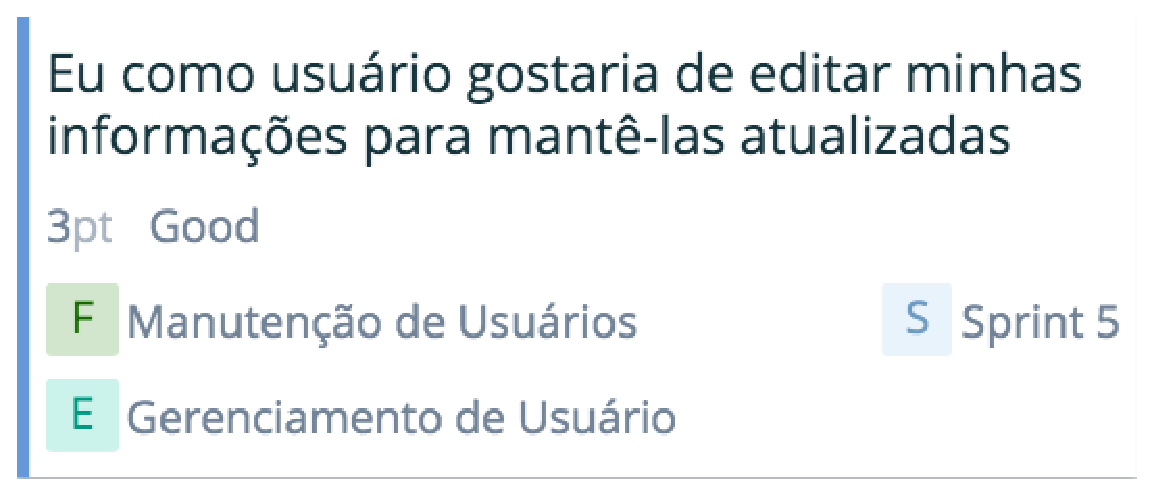
\includegraphics[keepaspectratio=true,scale=0.5]{figuras/time9.eps}
    \caption{História de Usuário 9}
    \label{fig:roadmap}
\end{figure}

\begin{figure}[H]
    \centering
	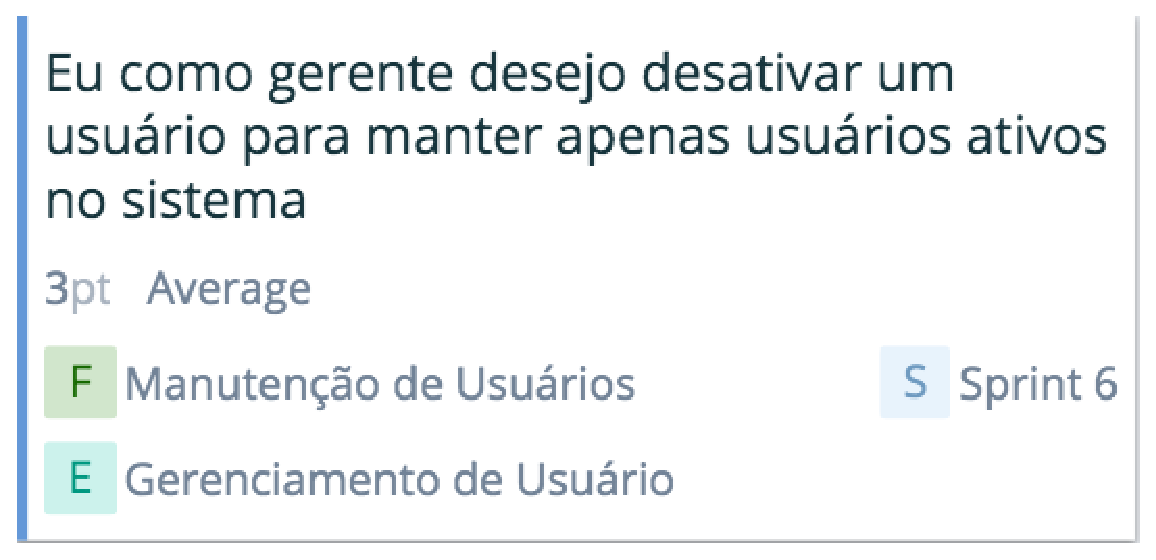
\includegraphics[keepaspectratio=true,scale=0.5]{figuras/time10.eps}
    \caption{História de Usuário 10}
    \label{fig:roadmap}
\end{figure}

\begin{figure}[H]
    \centering
	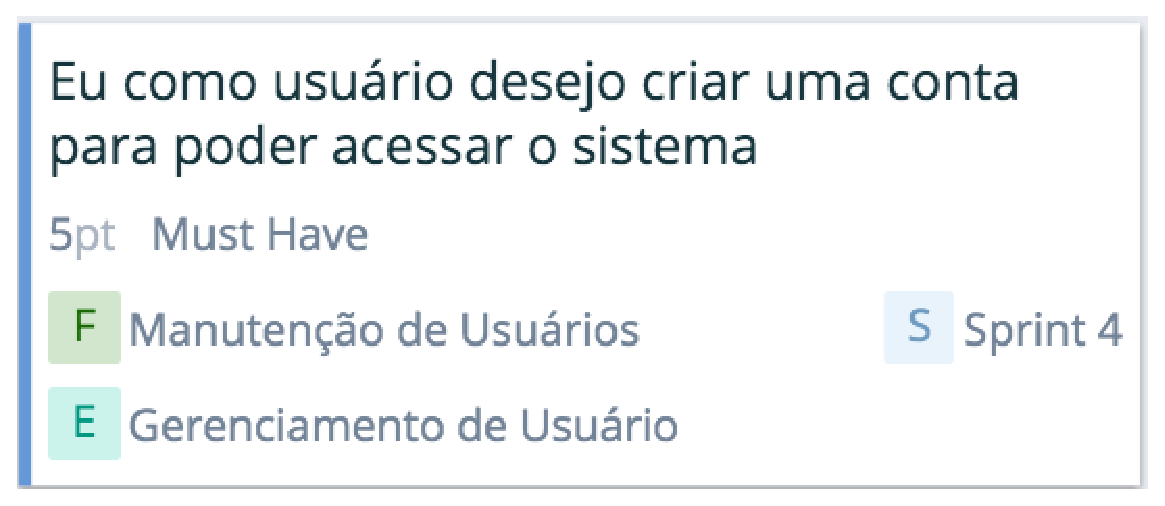
\includegraphics[keepaspectratio=true,scale=0.5]{figuras/time11.eps}
    \caption{História de Usuário 11}
    \label{fig:roadmap}
\end{figure}

\begin{figure}[H]
    \centering
	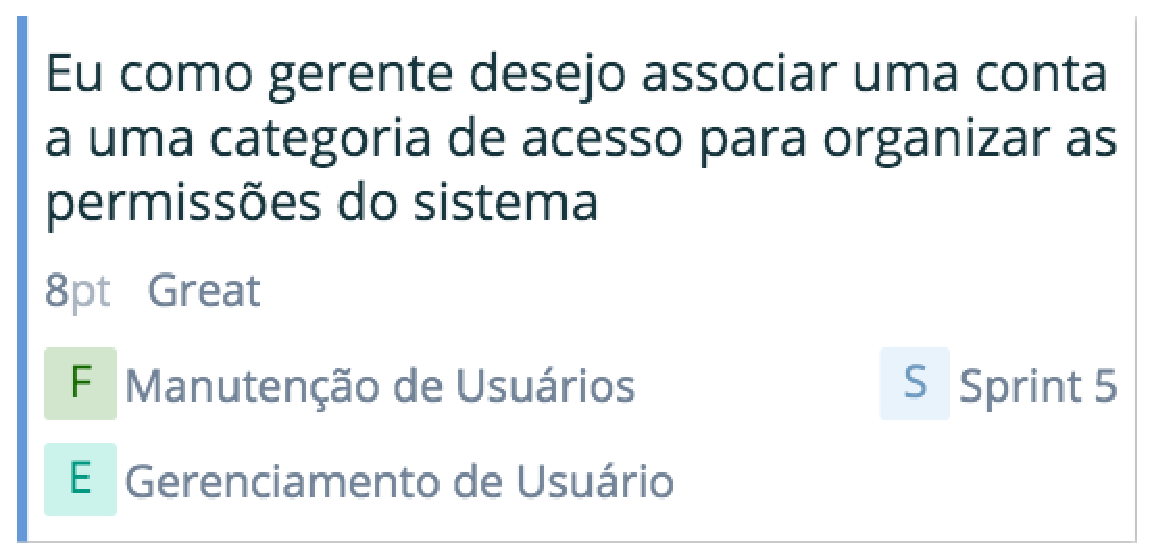
\includegraphics[keepaspectratio=true,scale=0.5]{figuras/time12.eps}
    \caption{História de Usuário 12}
    \label{fig:roadmap}
\end{figure}

Durate a \textbf{terceira} iteração do nível de programa, foram especificadas as seguintes histórias

\begin{figure}[H]
    \centering
	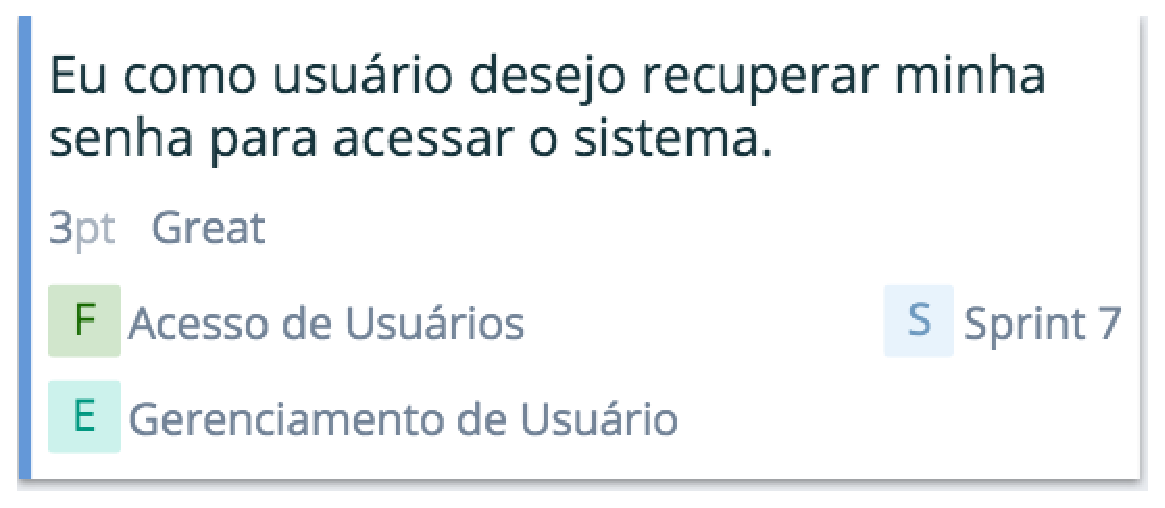
\includegraphics[keepaspectratio=true,scale=0.5]{figuras/time13.eps}
    \caption{História de Usuário 13}
    \label{fig:roadmap}
\end{figure}

\section{Gerência de Mudança}

\subsection{Atributos de Requisitos}

Atributos são uma fonte muito importante de informação sobre requisitos é a partir deles
que se sabe a origem, a sua importância relativa e a data em que foi criado.
Se criados apropriadamente, eles podem fornecer informações significantes sobre
o estado do sistema. Assim como é possível executar consultas para encontrar todos
os requisitos concluídos ou de alta prioridade.Dentre os tipos de atributos existentes,
foram utilizados:

\textbf{Benefício:} Indica o grau de benefício ou prioridade dos requisitos em relação às
expectativas dos Fornecedores de Requisitos.

\begin{figure}[H]
    \centering
	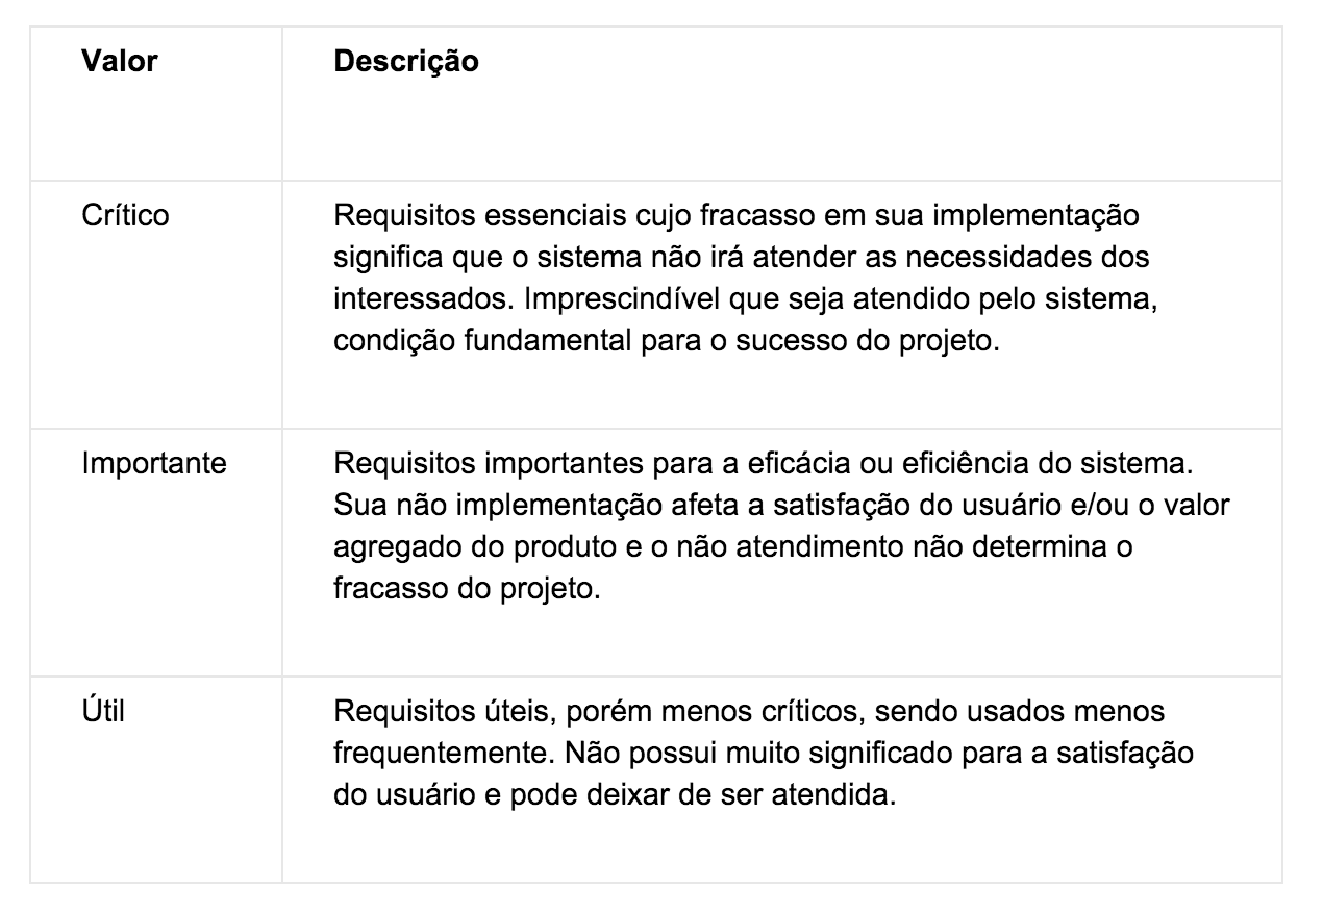
\includegraphics[keepaspectratio=true,scale=0.7]{figuras/atr1.eps}
    \caption{ Rastreabilidade Vertical de Portfolio na Ferramenta}
    \label{fig:ras}
\end{figure}

\textbf{Estabilidade:} Indica o grau de maturidade e confiabilidade em relação ao entendimento
e comprometimento de um requisito entre os envolvidos do projeto.

\begin{figure}[H]
    \centering
	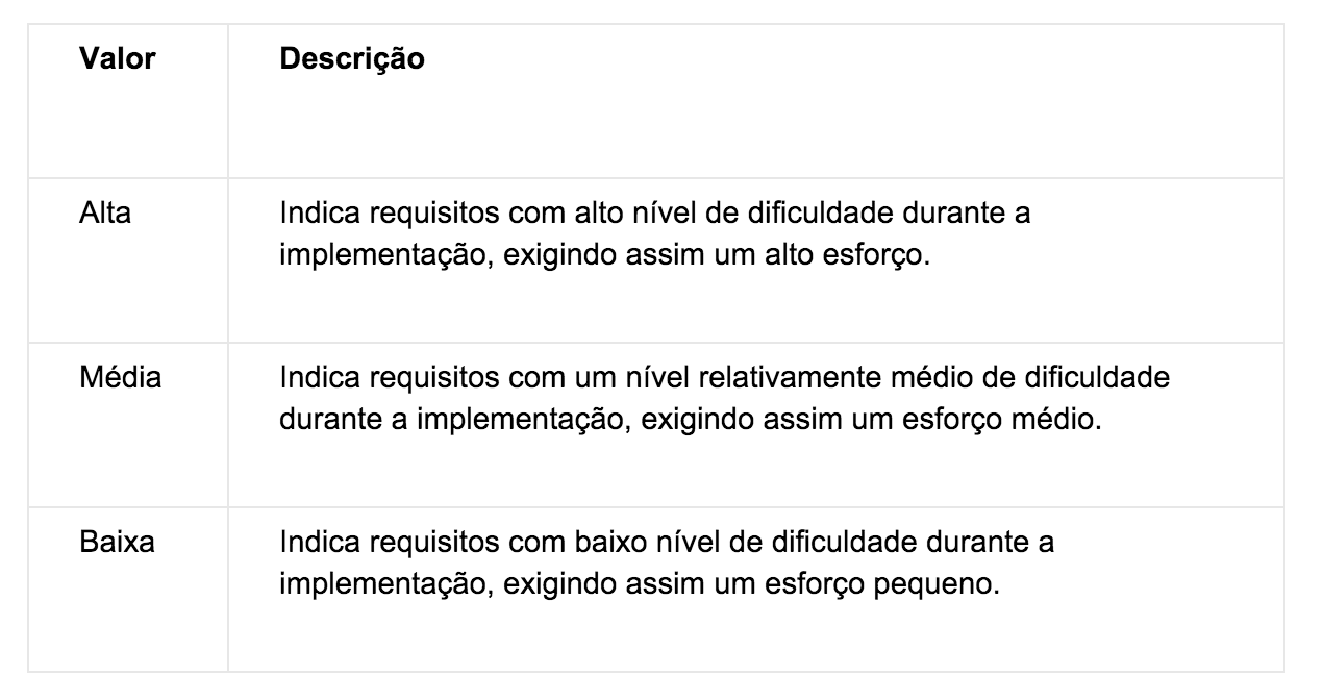
\includegraphics[keepaspectratio=true,scale=0.7]{figuras/atr3.eps}
    \caption{ Rastreabilidade Vertical de Portfolio na Ferramenta}
    \label{fig:ras}
\end{figure}

\textbf{Complexidade:} Indica o nível de esforço necessário ou o quão difícil é a implementação do requisito.

\begin{figure}[H]
    \centering
	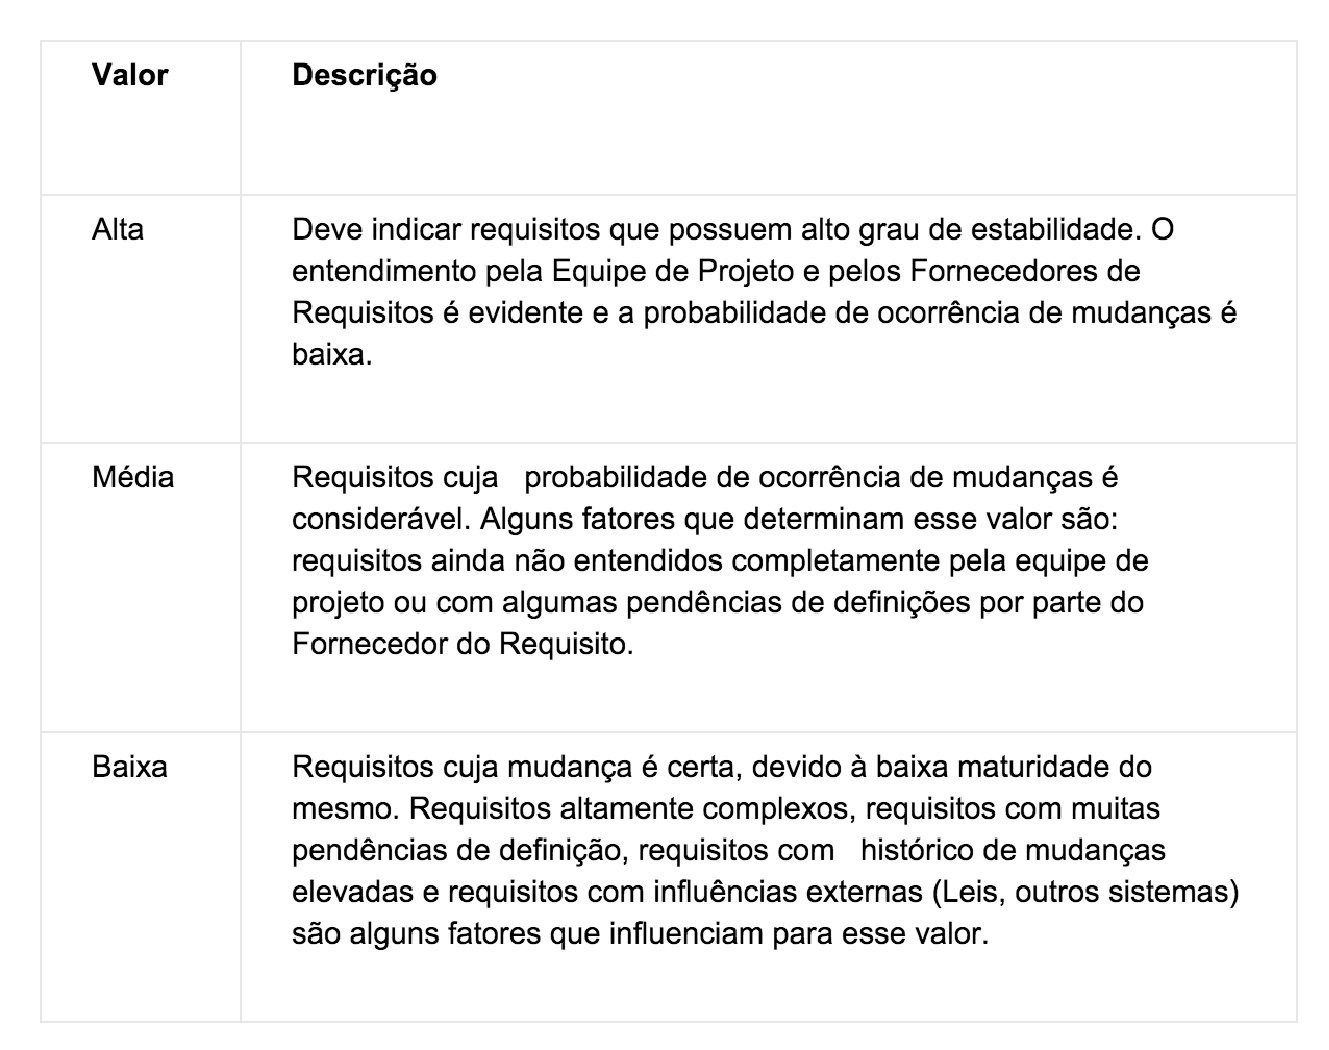
\includegraphics[keepaspectratio=true,scale=0.5]{figuras/atr10.eps}
    \caption{ Rastreabilidade Vertical de Portfolio na Ferramenta}
    \label{fig:ras}
\end{figure}

\textbf{Situação:} Indica a situação atual de um requisito.

\begin{figure}[H]
    \centering
	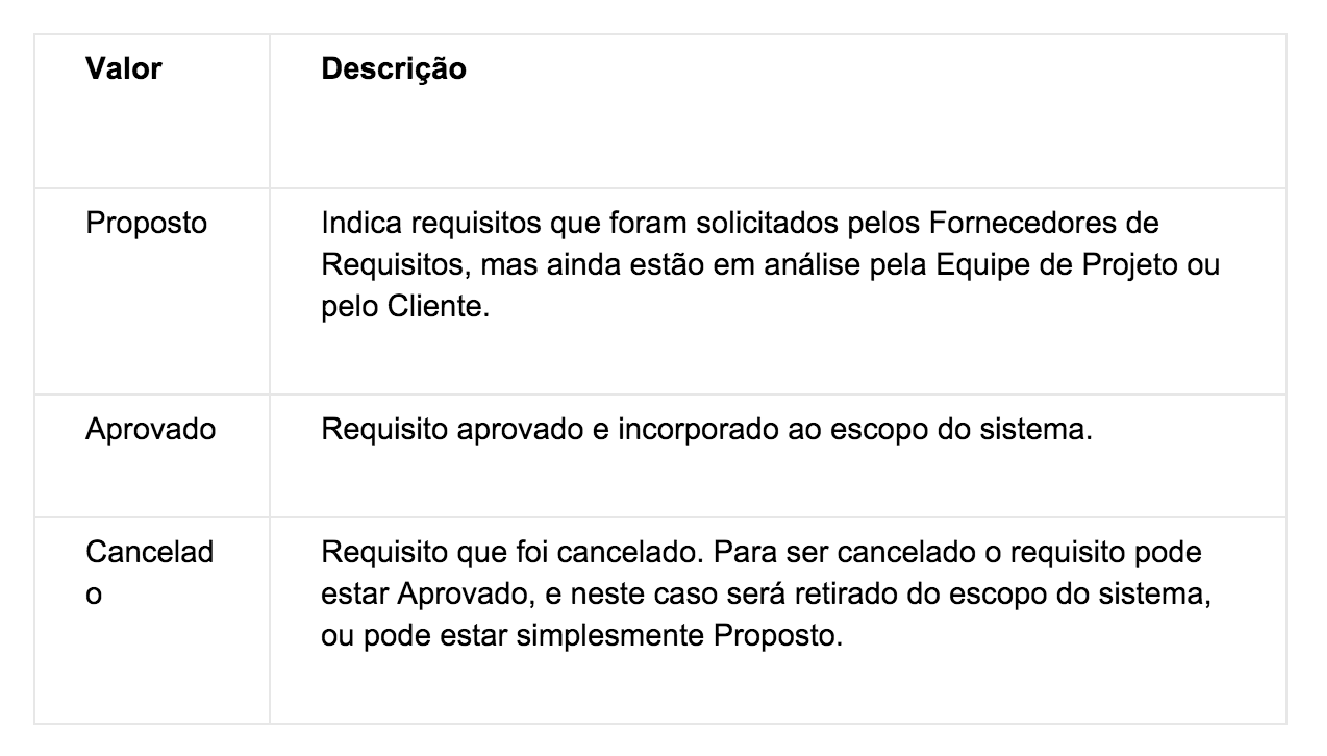
\includegraphics[keepaspectratio=true,scale=0.7]{figuras/atr4.eps}
    \caption{ Rastreabilidade Vertical de Portfolio na Ferramenta}
    \label{fig:ras}
\end{figure}

\textbf{Responsável:} Indica o nome do responsável na Equipe de Projeto pelo requisito.

\begin{figure}[H]
    \centering
	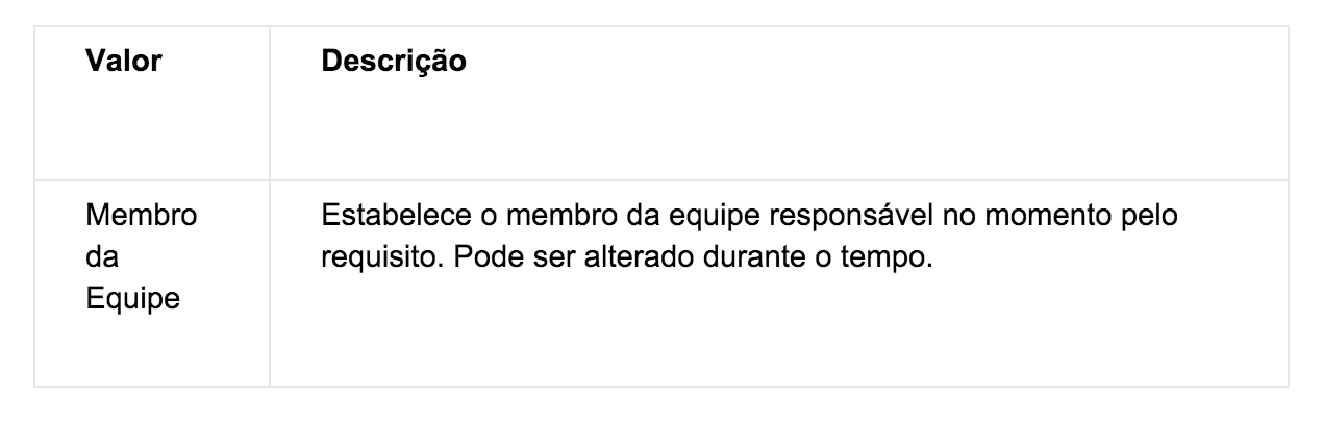
\includegraphics[keepaspectratio=true,scale=0.7]{figuras/atr5.eps}
    \caption{ Rastreabilidade Vertical de Portfolio na Ferramenta}
    \label{fig:ras}
\end{figure}

\textbf{Observações:} Atributo livre para registro de observações como pendências
ou problemas que atualmente está ocorrendo com o requisito.

\begin{figure}[H]
    \centering
	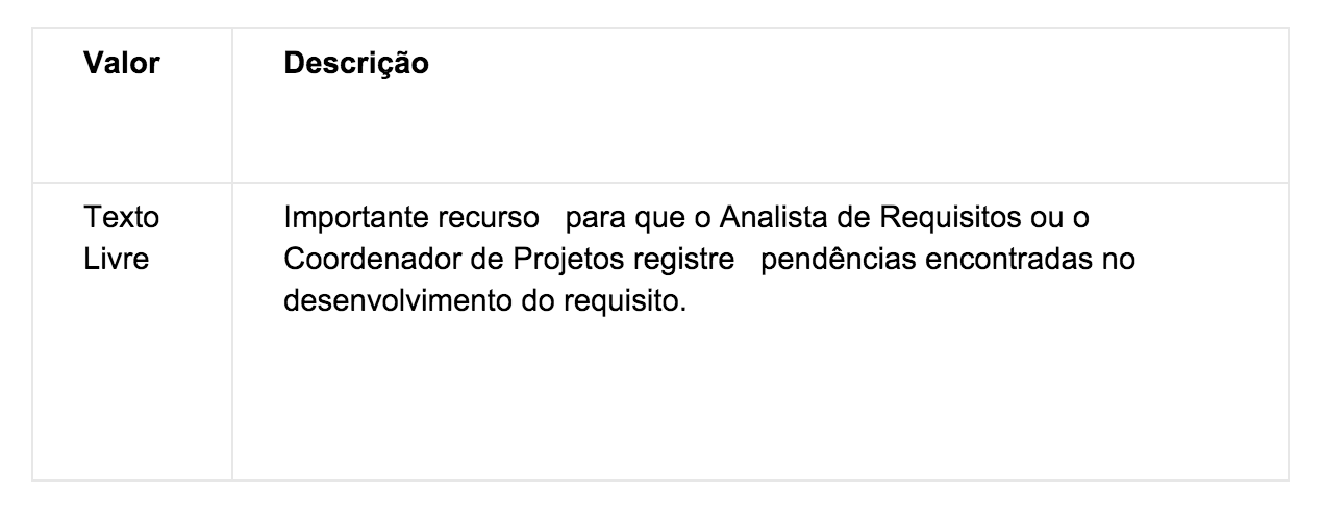
\includegraphics[keepaspectratio=true,scale=0.7]{figuras/atr6.eps}
    \caption{ Rastreabilidade Vertical de Portfolio na Ferramenta}
    \label{fig:ras}
\end{figure}

\subsection{Rastreabilidade de Requisitos}

Rastreabilidade é a propriedade de uma especificação de requisitos que reflete a facilidade
de encontrar os requisitos relacionados \cite{sommerville2007}.

Assim a rastreabilidade se torna vital a qualquer processo de software,
pois a partir de uma rastreabilidade bi-direcional descrita por \cite{DAVIS} sendo
a capacidade de rastrear um requisito até seus refinamentos é definida como rastrear
para frente (Forwards), e a de rastrear um refinamento até sua origem é definida como
rastrear para trás (Backwards) é possível rastrear objetos de origem/destino a partir de
qualquer ponto, refletindo a qualidade que \cite{PRIBERAM} diz: Denota a qualidade do
que é rastreável. A capacidade para acompanhar o percurso de um produto, ou de conhecer
o seu processo de produção, manipulação, transformação, embalagem ou expedição.

Assim, neste projeto tomamos como estratégia a rastreabilidade bi-direcional dos
requisitos, garantindo assim que a partir de um tema de investimento seja possível
rastrear todas as suas derivações, como ilustrado na figura \ref{fig:ras1} abaixo:

\begin{figure}[H]
    \centering
	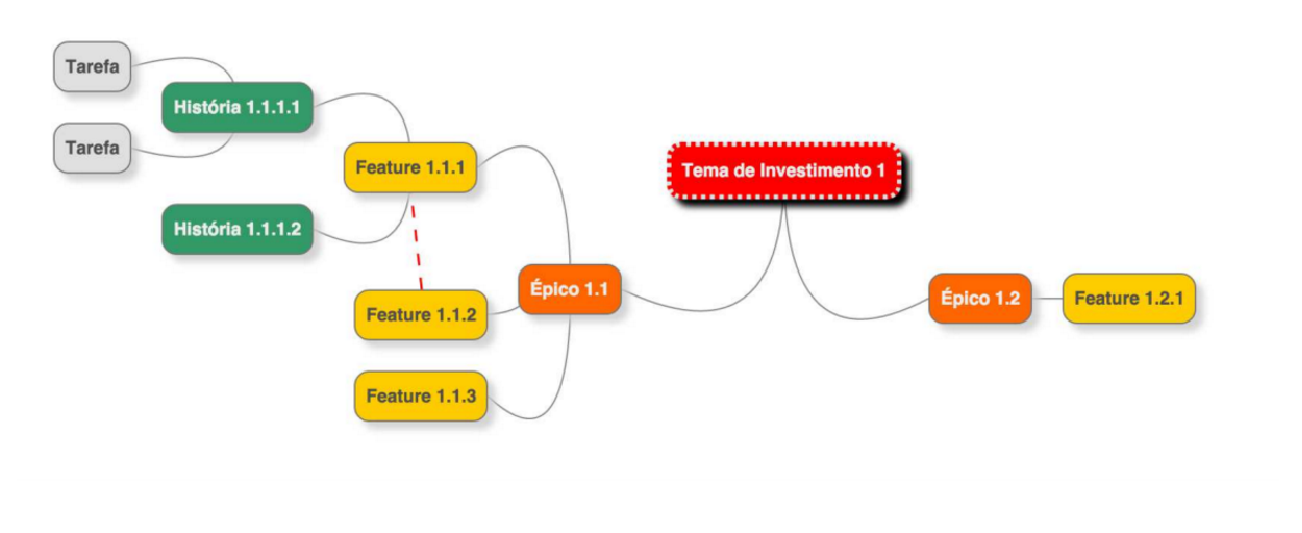
\includegraphics[keepaspectratio=true,scale=0.75]{figuras/rast1.eps}
    \caption{Visão geral da Rastreabilidade}
    \label{fig:ras1}
\end{figure}

As figuras abaixo mostram como a rastreabilidade é tratada na ferramente utilizada.

\begin{figure}[H]
    \centering
	\includegraphics[keepaspectratio=true,scale=0.75]{figuras/rast.eps}
    \caption{ Rastreabilidade Vertical de Portfolio na Ferramenta}
    \label{fig:ras}
\end{figure}

\begin{figure}[H]
    \centering
	\includegraphics[keepaspectratio=true,scale=0.5]{figuras/rast2.eps}
    \caption{Rastreabilidade Vertical de Programa na Ferramenta 1}
    \label{fig:ras2}
\end{figure}

\begin{figure}[H]
    \centering
	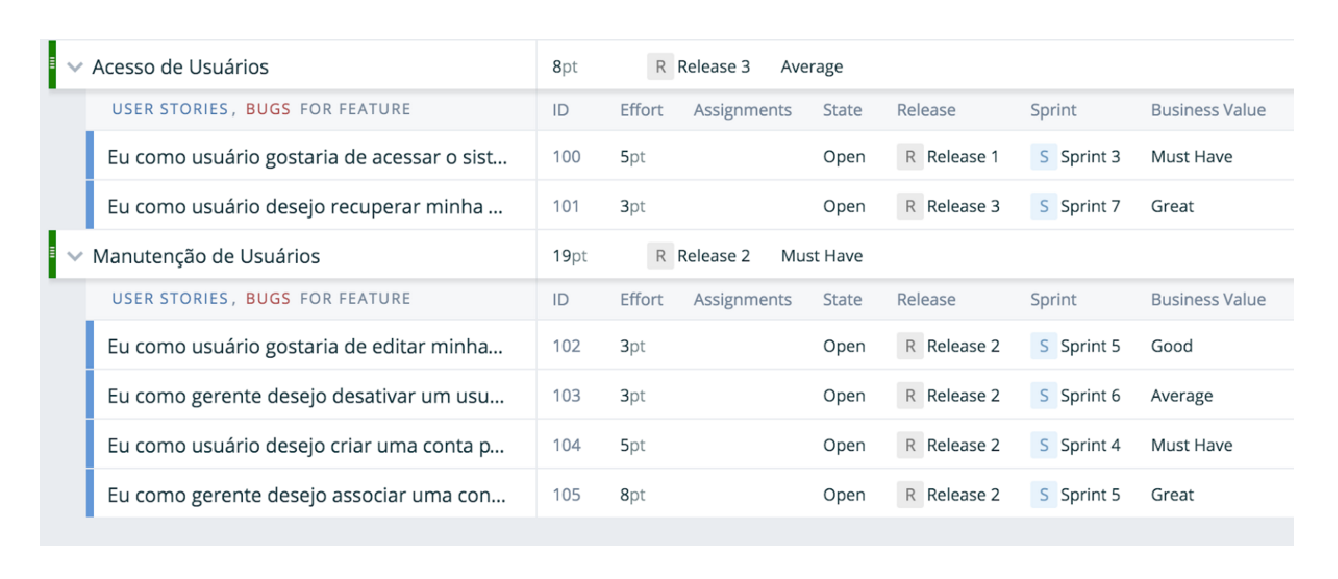
\includegraphics[keepaspectratio=true,scale=0.5]{figuras/fig1201.eps}
    \caption{Rastreabilidade Vertical de Programa na Ferramenta 2}
    \label{fig:ras2}
\end{figure}
